% Options for packages loaded elsewhere
\PassOptionsToPackage{unicode}{hyperref}
\PassOptionsToPackage{hyphens}{url}
%
\documentclass[
]{book}
\usepackage{lmodern}
\usepackage{amssymb,amsmath}
\usepackage{ifxetex,ifluatex}
\ifnum 0\ifxetex 1\fi\ifluatex 1\fi=0 % if pdftex
  \usepackage[T1]{fontenc}
  \usepackage[utf8]{inputenc}
  \usepackage{textcomp} % provide euro and other symbols
\else % if luatex or xetex
  \usepackage{unicode-math}
  \defaultfontfeatures{Scale=MatchLowercase}
  \defaultfontfeatures[\rmfamily]{Ligatures=TeX,Scale=1}
\fi
% Use upquote if available, for straight quotes in verbatim environments
\IfFileExists{upquote.sty}{\usepackage{upquote}}{}
\IfFileExists{microtype.sty}{% use microtype if available
  \usepackage[]{microtype}
  \UseMicrotypeSet[protrusion]{basicmath} % disable protrusion for tt fonts
}{}
\makeatletter
\@ifundefined{KOMAClassName}{% if non-KOMA class
  \IfFileExists{parskip.sty}{%
    \usepackage{parskip}
  }{% else
    \setlength{\parindent}{0pt}
    \setlength{\parskip}{6pt plus 2pt minus 1pt}}
}{% if KOMA class
  \KOMAoptions{parskip=half}}
\makeatother
\usepackage{xcolor}
\IfFileExists{xurl.sty}{\usepackage{xurl}}{} % add URL line breaks if available
\IfFileExists{bookmark.sty}{\usepackage{bookmark}}{\usepackage{hyperref}}
\hypersetup{
  pdftitle={Designcraft for experiments},
  pdfauthor={cjlortie},
  hidelinks,
  pdfcreator={LaTeX via pandoc}}
\urlstyle{same} % disable monospaced font for URLs
\usepackage{longtable,booktabs}
% Correct order of tables after \paragraph or \subparagraph
\usepackage{etoolbox}
\makeatletter
\patchcmd\longtable{\par}{\if@noskipsec\mbox{}\fi\par}{}{}
\makeatother
% Allow footnotes in longtable head/foot
\IfFileExists{footnotehyper.sty}{\usepackage{footnotehyper}}{\usepackage{footnote}}
\makesavenoteenv{longtable}
\usepackage{graphicx,grffile}
\makeatletter
\def\maxwidth{\ifdim\Gin@nat@width>\linewidth\linewidth\else\Gin@nat@width\fi}
\def\maxheight{\ifdim\Gin@nat@height>\textheight\textheight\else\Gin@nat@height\fi}
\makeatother
% Scale images if necessary, so that they will not overflow the page
% margins by default, and it is still possible to overwrite the defaults
% using explicit options in \includegraphics[width, height, ...]{}
\setkeys{Gin}{width=\maxwidth,height=\maxheight,keepaspectratio}
% Set default figure placement to htbp
\makeatletter
\def\fps@figure{htbp}
\makeatother
\setlength{\emergencystretch}{3em} % prevent overfull lines
\providecommand{\tightlist}{%
  \setlength{\itemsep}{0pt}\setlength{\parskip}{0pt}}
\setcounter{secnumdepth}{5}
\usepackage{booktabs}
\usepackage[]{natbib}
\bibliographystyle{apalike}

\title{Designcraft for experiments}
\author{cjlortie}
\date{2020-08-12}

\begin{document}
\maketitle

{
\setcounter{tocdepth}{1}
\tableofcontents
}
\hypertarget{introduction}{%
\chapter{Introduction}\label{introduction}}


\includegraphics[width=4in,height=\textheight]{./rabbit.png}

Welcome to experimental design. There are two sets of three exercises provided to explore principles for better experiments. This is a simple book to support the practical, at-home learning associated with experimental design. The text `Experimental Design for the Life Sciences' underpins the design principles \citep{RN6381}.

Life is an experiment. Individually and collectively. We experiment everyday. This is an opportunity to formalize some of those processes and make the learning from experimental design thinking a craft you can apply to all challenges. There are two primary modules to support this process.

\begin{enumerate}
\def\labelenumi{(\arabic{enumi})}
\item
  Field experiments comprises three outdoor experiments to explore sampling heterogeneous, complex processes in natural systems. The purpose is to provide choice. You need to try each, briefly, as a pilot experiment only. Then, select one to pursue in depth and write up as a research article.
\item
  The data experiments describe the opportunity to use design thinking to structure existing data that others have already collected. The same principles for better experiments still apply in how you reuse the data. There are also three examples provided. Select only one and write up as a note.
\end{enumerate}

Both report formats supported by \href{https://www.facetsjournal.com/about/}{FACETS}. It is the first and only open access science journal in Canada.

\hypertarget{workflow-for-pilot-and-field-experiment}{%
\subsubsection*{Workflow for pilot and field experiment}\label{workflow-for-pilot-and-field-experiment}}
\addcontentsline{toc}{subsubsection}{Workflow for pilot and field experiment}

\begin{enumerate}
\def\labelenumi{\arabic{enumi}.}
\tightlist
\item
  Do all three field experiments in brief, pilot only, try each for a few hours each.
\item
  Then, Select one of the first three field experiments to publish data with meta-data.\\
\item
  Publish your data with meta-data to an open and public data repository such as \href{https://figshare.com}{figshare}.\\
\item
  Share the link with all the files with the teaching assistment via the course turnitin.com platform.\\
\item
  Select one of the three field experiments to do a deeper dive, i.e.~fuller experiment wherein you structure observation by a key variable in the environment.\\
\item
  Design experiment, collect data for the deeper dive.\\
\item
  Consider combining data from other students that examined the same system.
\item
  Publish data with meta-data to \href{https://figshare.com}{figshare} and submit to teaching assistant via \href{https://www.turnitin.com}{turnitin.com}.\\
\item
  Write up the field experiment you completed for the deeper dive as a research article for the Canadian open science journal \href{https://www.facetsjournal.com/authors/instructions/}{Facets}.\\
\item
  Submit paper to teaching assistant via \href{https://www.turnitin.com}{turnitin.com}.
\end{enumerate}

\hypertarget{workflow-for-the-data-design-lab-report}{%
\subsubsection*{Workflow for the data-design lab report}\label{workflow-for-the-data-design-lab-report}}
\addcontentsline{toc}{subsubsection}{Workflow for the data-design lab report}

\begin{enumerate}
\def\labelenumi{\arabic{enumi}.}
\tightlist
\item
  Explore each dataset.\\
\item
  Plan a variable to structure your design and analysis.\\
\item
  Reuse the data to explore your hypothesis and test your predictions.\\
\item
  Write a short research `note' format paper suitable for publication in \href{https://www.facetsjournal.com/authors/instructions/}{Facets journal}.\\
\item
  Submit paper to teaching assistant via \href{https://www.turnitin.com}{turnitin.com}.
\end{enumerate}

\hypertarget{field-experiments-gear-and-prep}{%
\subsubsection*{Field experiments gear and prep}\label{field-experiments-gear-and-prep}}
\addcontentsline{toc}{subsubsection}{Field experiments gear and prep}

\hypertarget{data-design-experiment-prerequisites}{%
\subsubsection*{Data-design experiment prerequisites}\label{data-design-experiment-prerequisites}}
\addcontentsline{toc}{subsubsection}{Data-design experiment prerequisites}

\hypertarget{birds}{%
\chapter{Balcony birdwatching}\label{birds}}


\includegraphics[width=4in,height=\textheight]{./owl.png}\\
Bird observation, from a distance.

\hypertarget{learning-outcomes}{%
\subsubsection*{Learning outcomes}\label{learning-outcomes}}
\addcontentsline{toc}{subsubsection}{Learning outcomes}

\begin{enumerate}
\def\labelenumi{\arabic{enumi}.}
\tightlist
\item
  Identify common species of birds locally.\\
\item
  Collect a dataset.\\
\item
  Connect principles of experimental design to implementation.\\
\item
  Write clear and reusable meta-data.\\
\item
  Contribute to open science by publishing data and meta-data.
\end{enumerate}

\hypertarget{steps}{%
\subsubsection*{Steps}\label{steps}}
\addcontentsline{toc}{subsubsection}{Steps}

\begin{enumerate}
\def\labelenumi{\arabic{enumi}.}
\tightlist
\item
  Scout out a location with more than a single species of birds and a frequency of a few different individuals of birds over a 5-10 minute duration.\\
\item
  Select a good spot to the observe birds at your designated location. It can be a balcony or quiet spot. Vegetation such as trees or shrubs can facilitate observation of birds by providing habitat.\\
\item
  Choose a distance that permits enough resolution to see plumage and what an individual bird is doing (depending on whether you are using binoculars, a spotting scope, or unassisted with your vision). There are considerable merits to observing birds more simply \citep{RN6773}. You are also welcome to address any visibility or spotting challenges using bird calls to record frequency of birds in a sampling region.\\
\item
  Specify a duration to sample, for instance, 60 minutes when you have observed the most birds in your scouting exercise. Remember, this is a pilot experiment. Take qualitative notes, sketch, and complete this datasheet.\\
\item
  Use your notes to complete a meta-data file, i.e.~a description of how the data were collected, whether, when, and what each attribute in your dataset means.\\
\item
  Sign out a bird guide for your region from the library or university or try out a \href{https://www.birds.cornell.edu/k12/best-apps-for-birding-with-kids/}{free app} for now to support identification.
\end{enumerate}

\hypertarget{data}{%
\subsubsection*{Data}\label{data}}
\addcontentsline{toc}{subsubsection}{Data}

\href{https://figshare.com/articles/dataset/BIOL3250_birds_datasheet/12756101}{Here} is a sample datasheet for the pilot experiment. This is set up as species-level observations, i.e.~each row or replicate is a species of bird you observe. This datasheet is for the pilot experiment, and it is a stepping stone for the deeper dive experiment if you choose to complete this experiment for your first report. A more detailed datasheet can consider duration or start and stop times of each individual bird, more details on the environment, or record interesting ecological or environmental variables that are present in the environment too - noise, disturbance, squirrels, other birds, etc.

Data can be organized in many different formats depending on the approach to collecting the data in the field or the lab, the instrument or method used, preference, or accepted standards within the domain of study. In many modern data science endeavours, data are also formatted according to the principles of `tidy data' \citep{RN4416}. The following three rules define data as tidy \citep{RN4369}.

\begin{enumerate}
\def\labelenumi{\arabic{enumi}.}
\tightlist
\item
  Each variable must have its own column.\\
\item
  Each observation must have its own row.\\
\item
  Each value must have its own cell.
\end{enumerate}

Most scripting languages such as \href{https://www.r-project.org}{R} or \href{https://www.python.org}{Python} can resolve and tidy up data to adhere to these principles, but with a little planning, your data can be set up to facilitate this process and enable easier data visualization and models.

\textbf{Sample data set}\\
In this example, the field observations were coded as one species per behaviour per row. A compromise between tidiness and ease of collecting the tallies per species in the field.

\begin{tabular}{rllllrl}
\toprule
rep & date & researcher & location & species & frequency & behaviour\\
\midrule
1 & 15/9/2020 & cl & High Park, Toronto & House sparrow & 12 & flying\\
2 & 15/9/2020 & cl & High Park, Toronto & Blue jay & 2 & foraging\\
3 & 15/9/2020 & cl & High Park, Toronto & Cedar waxwing & 1 & perching\\
4 & 15/9/2020 & cl & High Park, Toronto & Cedar waxwing & 3 & foraging\\
5 & 15/9/2020 & cl & High Park, Toronto & Dark-eyed junco & 2 & flying\\
\addlinespace
6 & 15/9/2020 & cl & High Park, Toronto & Black-capped Chickadee & 3 & foraging\\
7 & 15/9/2020 & cl & High Park, Toronto & Black-capped Chickadee & 2 & posturing\\
8 & 15/9/2020 & cl & High Park, Toronto & Black-capped Chickadee & 3 & interacting with another bird\\
9 & 15/9/2020 & cl & High Park, Toronto & Black-capped Chickadee & 2 & sitting\\
10 & 15/9/2020 & cl & High Park, Toronto & Wood thrush & 2 & flying\\
\addlinespace
11 & 15/9/2020 & cl & High Park, Toronto & Wood thrush & 5 & on ground\\
12 & 15/9/2020 & cl & High Park, Toronto & Northern flicker & 1 & perching in a tree\\
\bottomrule
\end{tabular}

\hypertarget{meta-data}{%
\subsubsection*{Meta-data}\label{meta-data}}
\addcontentsline{toc}{subsubsection}{Meta-data}

In many disciplines of science, meta-data are the descriptive elements of the dataset. They provide a clear means for discovery and reuse of data collected - by you in future and for others \citep{RN3201, RN6774}. For the purposes of our practical learning in experimental design here, describe what each column in our dataset means, describe the structure of your dataset (i.e.~each row is a species-level observation, or plot, or transect), describe the duration of sampling, location, and provide a bit of guidance for someone to use in inspecting the dataset. It is very similar to the methods in conventional publications or standard reports, but it ensures each attribute in the dataset has a brief description. It is also superb preparation for the methods if you choose to write a report.

\hypertarget{deeper-dive}{%
\subsubsection*{Deeper dive}\label{deeper-dive}}
\addcontentsline{toc}{subsubsection}{Deeper dive}

If you choose this adventure, your goal is to experiment with the method of animal observation to test a hypothesis and predictions. The text `Experimental Design for the Life Sciences' does an excellent job of explaining how to set up hypotheses and predictions \citep{RN6381}. Pilot experiment first, think, explore your data and notes, then write your ideas down that you want to test. A hypothesis is a clear explanation of how a system works \citep{RN6776, RN6775}. The predictions are logical and reasonable outcomes if the hypothesis is a good approximation of how the system works, i.e.~the key variables that make it work. Predictions should be testable and read like simple sentences that describe results. The goal of the deeper-dive experiment is to take your pilot experiment, examine what worked and did not work so well in your experiment, and do a deeper and more thorough job of testing a key idea that you are interested in associated with bird communities in your backyard or neighbourhood. The goal should be to explore one key factor that describes how the species locally interact within one another, the environment or other species, or resources.

\hypertarget{bioblitz}{%
\chapter{Backyard bioblitz}\label{bioblitz}}


\includegraphics[width=4in,height=\textheight]{./insects.png}

A \href{https://en.wikipedia.org/wiki/BioBlitz}{bioblitz} is a biodiversity survey that is done rapidly for a specific place. National Geographic provides an excellent `getting started' \href{https://media.nationalgeographic.org/assets/file/NationalGeographicBioBlitzGuide.pdf}{guide} to the process.

\hypertarget{learning-outcomes}{%
\subsubsection*{Learning outcomes}\label{learning-outcomes}}
\addcontentsline{toc}{subsubsection}{Learning outcomes}

\begin{enumerate}
\def\labelenumi{\arabic{enumi}.}
\tightlist
\item
  Identify common species of animals locally.\\
\item
  Collect a dataset.\\
\item
  Connect principles of experimental design to implementation.\\
\item
  Write clear and reusable meta-data.\\
\item
  Contribute to open science by publishing data and meta-data.
\end{enumerate}

\hypertarget{steps}{%
\subsubsection*{Steps}\label{steps}}
\addcontentsline{toc}{subsubsection}{Steps}

\begin{enumerate}
\def\labelenumi{\arabic{enumi}.}
\tightlist
\item
  Scout out a location that has a few species of animals. Vertebrate or invertebrate taxa - preferably both. A medium-size backyard, park, woodlot, or grassland is ideal.\\
\item
  Do a bioblitz or intensive process of surveying a specific place for a short duration of time to estimate all the living species (excepting plants) locally.\\
\item
  For the purposes of this experiment, focus on on all animals you can spot.\\
\item
  Select a set of locations within the designated area to sample. This can include direct observation of species spots, a region, walking through a region repeatedly. Select the scale carefully that matches what you can observe. This can be relatively unstructured sampling process with the goal of documenting as many species as possible that reside in this place.\\
\item
  Record your data to your datasheet and also consider using the \href{https://www.inaturalist.org}{iNaturalist} free app to record and share your observations globally.
\end{enumerate}

\hypertarget{data}{%
\subsubsection*{Data}\label{data}}
\addcontentsline{toc}{subsubsection}{Data}

\href{https://figshare.com/articles/dataset/BIOL3250_bioblitz_datasheet/12792455}{Here} is a sample datasheet for the pilot experiment. This is set up as species-level observations, i.e.~each row is replicate species you observe. This datasheet is not structured for frequency or density - simply a comprehensive list of all animal species you can spot during the pilot experiment.

\hypertarget{meta-data}{%
\subsubsection*{Meta-data}\label{meta-data}}
\addcontentsline{toc}{subsubsection}{Meta-data}

Describe how you collected the data. Ensure that each attribute in the dataset has a brief description. This is like an abbreviated version of the methods section in peer-reviewed science publications. Report total sampling time and any relevant details that enable someone else to reuse these data or repeat the process of doing a bioblitz that collecting similar data in a different place.

\hypertarget{deeper-dive}{%
\subsubsection*{Deeper dive}\label{deeper-dive}}
\addcontentsline{toc}{subsubsection}{Deeper dive}

If you choose this adventure, your goal is to experiment with the method of measuring biodiversity locally. Innovate on the pilot experiment, simple biodiversity inventory methodology to test a hypothesis and predictions. The predictions should be logical and reasonable outcomes if the hypothesis is a good approximation of how the system works, i.e.~the key variables that make it work. Predictions should be testable and read like simple sentences that describe results. The goal of the deeper-dive experiment is to take your pilot experiment, examine what worked and did not work so well in your experiment, and do a deeper and more thorough job of testing a key idea that you are interested in associated with biodiversity patterns locally. The goal should be to explore one key factor that describes why biodiversity varies locally - at the scale you define.

\hypertarget{survey}{%
\chapter{Solo surveys}\label{survey}}

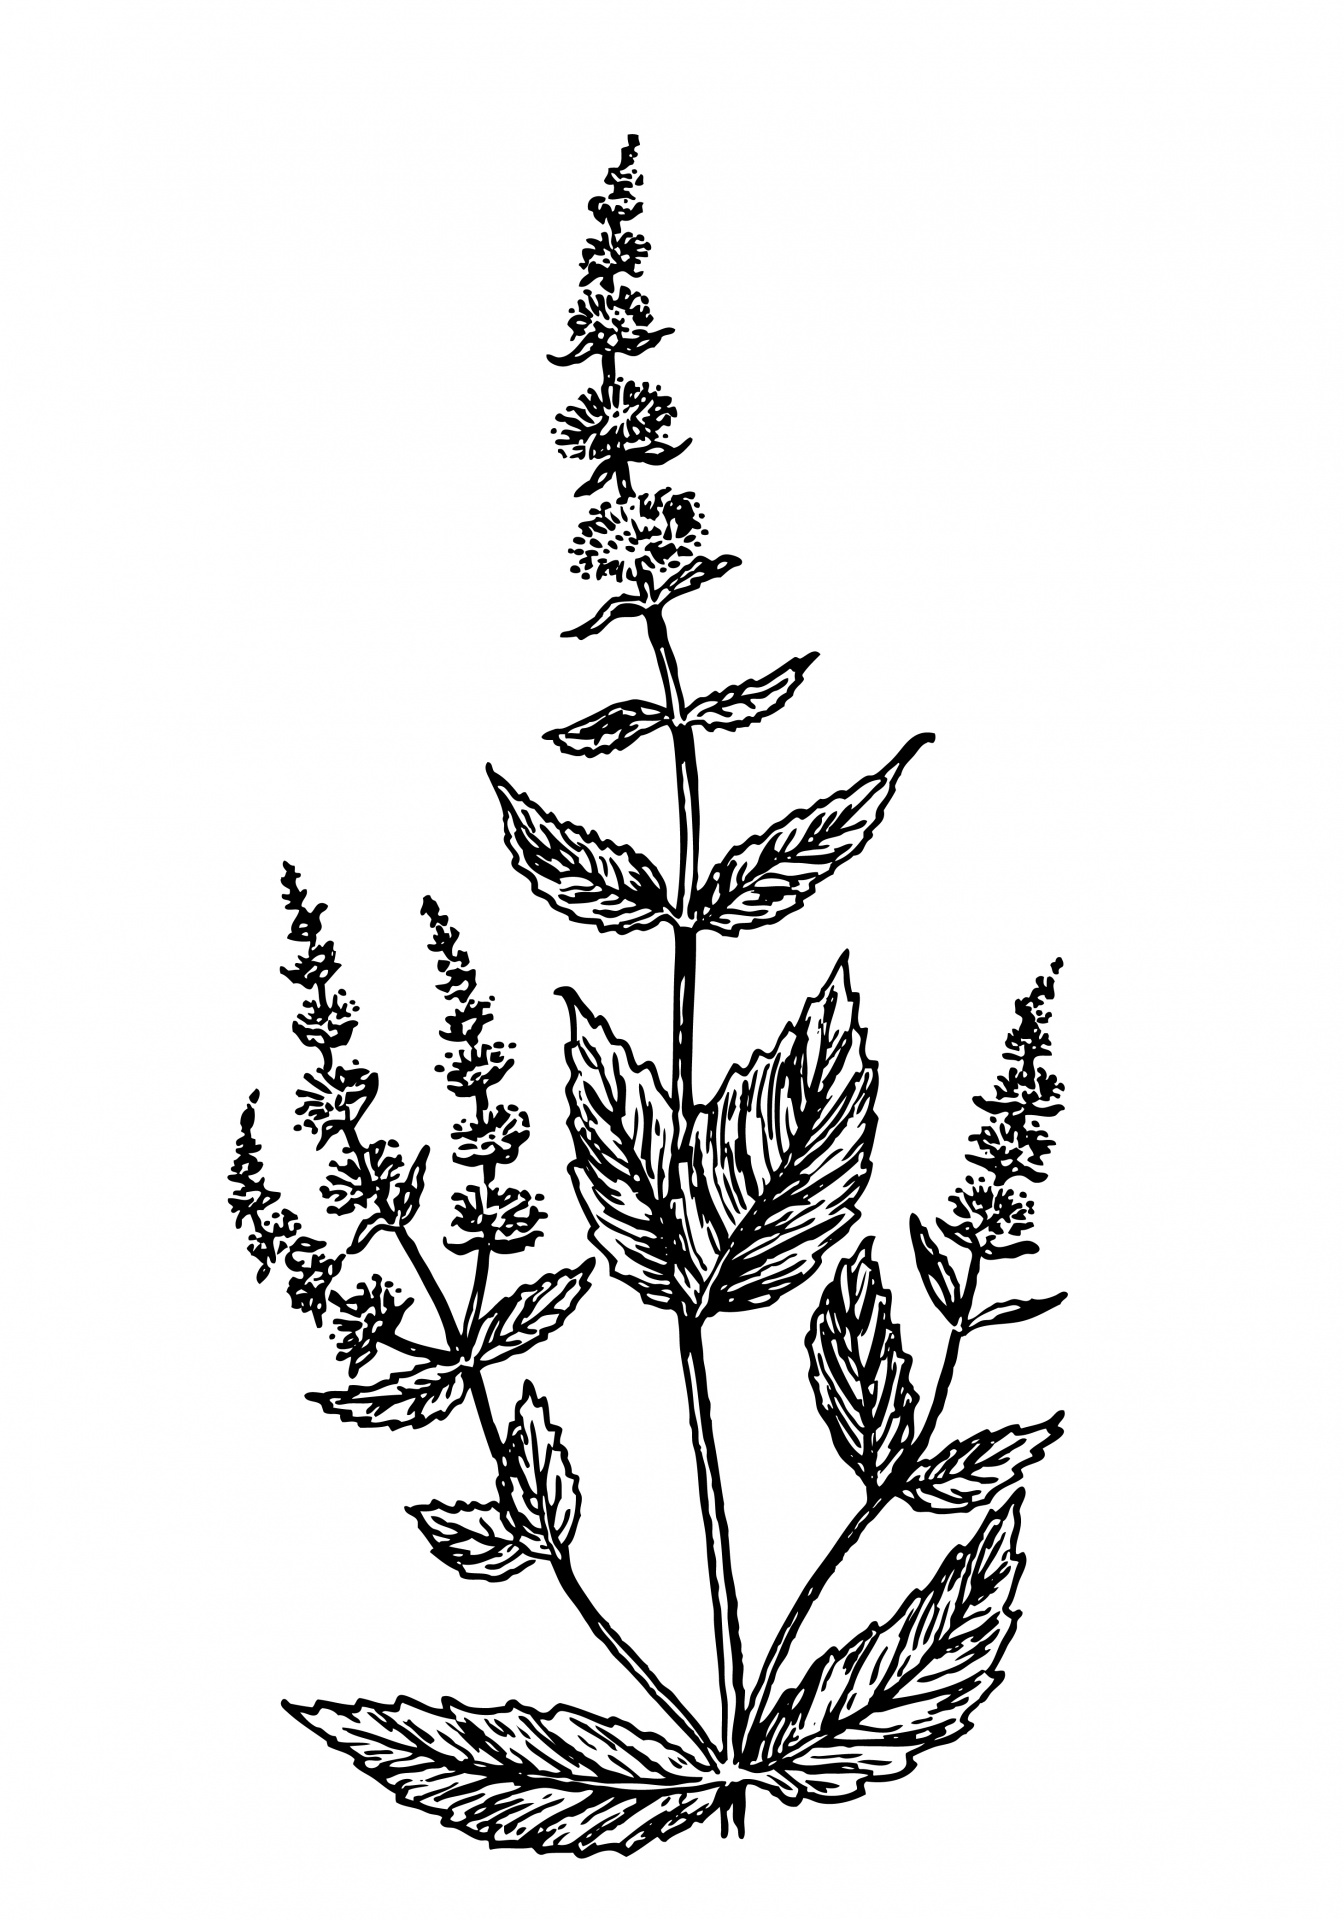
\includegraphics[width=4in,height=\textheight]{./plant.jpg}

Distributed ecological networks often use surveys done by individuals or small-teams to compile data on species or communities. Transects and quadrats are typically used to structure these `walk-through' surveys to estimate abundances and distributions of focal species. In this experiment, plants are examined.

\hypertarget{learning-outcomes}{%
\subsubsection*{Learning outcomes}\label{learning-outcomes}}
\addcontentsline{toc}{subsubsection}{Learning outcomes}

\begin{enumerate}
\def\labelenumi{\arabic{enumi}.}
\tightlist
\item
  Appreciate the complexity of plant communities.\\
\item
  Collect a dataset.\\
\item
  Connect principles of experimental design to implementation.\\
\item
  Write clear and reusable meta-data.\\
\item
  Contribute to open science by publishing data and meta-data.
\end{enumerate}

\hypertarget{steps}{%
\subsubsection*{Steps}\label{steps}}
\addcontentsline{toc}{subsubsection}{Steps}

\begin{enumerate}
\def\labelenumi{\arabic{enumi}.}
\tightlist
\item
  Select a location that has at least 50m of space to walk a straight line unimpeded. This can be a forest, lot, disturbed area, grassland, or even a parking lot with enough cracks and permeable spots for plants to grow.\\
\item
  Run out a piece of string, rope, or just measure 1m and line it up visually for a total length of 50m.\\
\item
  Every meter, place a 0.5m quadrat or 0.5 by 0.5m square (string, ruler, cardboard, pvc pipe, measured piece of bamboo) on the ground.\\
\item
  Record the total number of different plant species present (i.e.~species richness).\\
\item
  Estimate the total cover of all plants within the quadrat from 0 to 100\% cover.
\end{enumerate}

\hypertarget{data}{%
\subsubsection*{Data}\label{data}}
\addcontentsline{toc}{subsubsection}{Data}

\href{https://figshare.com/articles/dataset/BIOL3250_survey_datasheet/12792482}{Here} is a sample datasheet for the pilot experiment. This is set up as plot-level observations, i.e.~each row is replicate plot, one for each meter sampled on the 50m transect or line. This datasheet is structured very coarsely to estimate the total number of plant species and total cover of vegetation within the plots.

\hypertarget{meta-data}{%
\subsubsection*{Meta-data}\label{meta-data}}
\addcontentsline{toc}{subsubsection}{Meta-data}

Describe how you collected the data. Ensure that each attribute in the dataset has a brief description. This is like an abbreviated version of the methods section in peer-reviewed science publications.

\hypertarget{deeper-dive}{%
\subsubsection*{Deeper dive}\label{deeper-dive}}
\addcontentsline{toc}{subsubsection}{Deeper dive}

If you choose this adventure, your goal is to experiment with the method of measuring plant communities. Innovate on the pilot experiment design and add more depth to your quantitative description of the plant community. These innovations can include deeper insights into the structure of the community (height of plants, density of all plants, or spatial patterns) or the composition (i.e.~species identity, abundance per species per plot, flowering or not, native or invasive, or by plant functional groups). The predictions should be logical and reasonable outcomes if the hypothesis is a good approximation of how the system works, i.e.~the key variables that make it work. Predictions should be testable and read like simple sentences that describe results. The goal of the deeper-dive experiment is to take your pilot experiment, examine what worked and did not work so well in your experiment, and do a deeper and more thorough job of testing a key idea that you are interested in associated with biodiversity patterns locally. The goal should be to explore one key factor that can be used to describe or predict plant community structure or composition for the specific habitat sampled.

\hypertarget{magic}{%
\chapter{Magic data}\label{magic}}

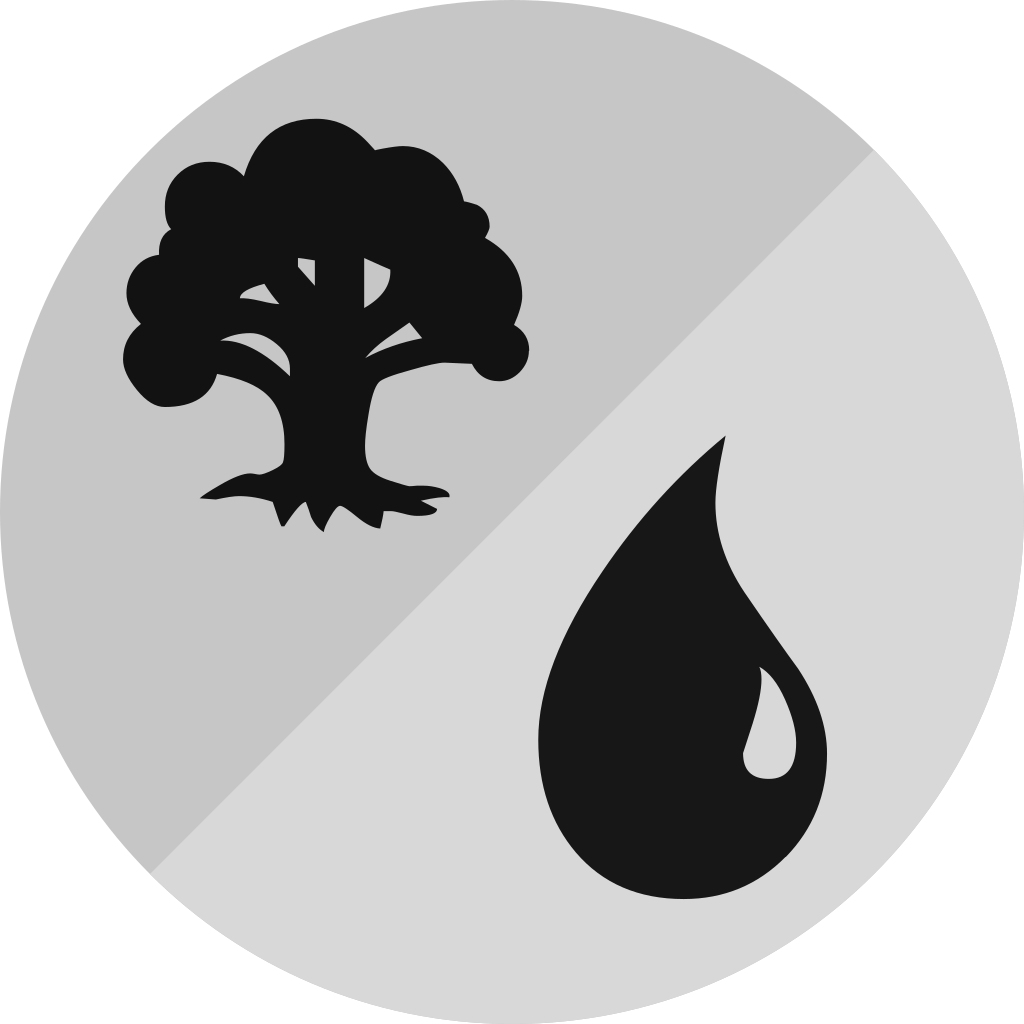
\includegraphics[width=4in,height=\textheight]{./magic.png}

\href{https://magic.wizards.com/en}{Magic: The Gathering} is a popular collectible card game that includes strategy and chance. If you have not played, here is a great \href{https://en.wikipedia.org/wiki/Magic:_The_Gathering}{description}. This is an excellent example of data collected that is appropriate for experimentation for several reasons. Many games have expansion packs and add-ons. Physical card collecting from sports to fantasy is a very popular activity in addition to a \href{https://www.nytimes.com/2018/03/23/your-money/trading-cards-investment.html}{multi-million dollar} economy and sales continue to \href{https://www.forbes.com/sites/chriscason/2020/05/28/why-the-sports-card-industry-has-not-yet-reached-its-peak/\#763af2e31fb7}{grow}. Consequently, these data are an opportunity to explore likelihood and consumer buying choices. It is also fun. Incidentally, the most valuable card reportedly sold for \href{https://screenrant.com/magic-the-gathering-most-rare-expensive-valuable-cards/}{\$250,000USD} so understanding how frequently rare cards pops up is pretty interesting.

\hypertarget{learning-outcomes}{%
\subsubsection*{Learning outcomes}\label{learning-outcomes}}
\addcontentsline{toc}{subsubsection}{Learning outcomes}

\begin{enumerate}
\def\labelenumi{\arabic{enumi}.}
\tightlist
\item
  Work with an existing dataset and reuse it.\\
\item
  Design questions from data.\\
\item
  Connect principles of experimental design to implementation with data.\\
\item
  Write a clear hypothesis and predictions to explain or predict patterns in data.\\
\item
  Communicate data, design, and science succinctly.
\end{enumerate}

\hypertarget{steps}{%
\subsubsection*{Steps}\label{steps}}
\addcontentsline{toc}{subsubsection}{Steps}

\begin{enumerate}
\def\labelenumi{\arabic{enumi}.}
\tightlist
\item
  Download the dataset.\\
\item
  Read the meta-data, and review what the game involves.\\
\item
  Explore likelihood topics, and prep a list of questions for the data.
\item
  Test one question with the data via a plot and a statistical test.\\
\item
  Decide if this is the dataset for you to write up as short research note.
\end{enumerate}

\hypertarget{data}{%
\subsubsection*{Data}\label{data}}
\addcontentsline{toc}{subsubsection}{Data}

\href{https://figshare.com/articles/dataset/Magic_The_Gathering_Data/12797474}{Here} are the data collected by a researcher at York University. These data are the first of their kind and super fascinating.

\hypertarget{deeper-dive}{%
\subsubsection*{Deeper dive}\label{deeper-dive}}
\addcontentsline{toc}{subsubsection}{Deeper dive}

If you choose this adventure, your goal is to explore any component of the data to apply design principles. Informally, we are data mining \citep{RN6800}. Data mining is a field of data science and many other disciplines that is exploding in capacity and application \citep{RN6802, RN6801}. Typically, mining data includes seeking patterns and building models that either focus on description or on prediction. Experimental design principles are not always a component of data mining endeavours, and this is unfortunate. We can do better science and build better models with design thinking principles. It is still an experiment, but someone else (or you) collected data. Data can be used for the explicit purpose they were collected, re-purposed to explore another idea, or simply collected without a priori hypotheses and predictions that we derive later. This is where design thinking can make profound contributions. Select a variable from the data that you think can be a meaningful mechanism or explains patterns, describe differences, or predict outcomes. In this example, this design and experimentation process can include good thinking and data use to examine price prediction, likelihood of rares or other card categories, and pattern frequencies by various card attributes. Begin with one key variable that can be a factor or grouping variable and one key variable that is a response or outcome. Then, do some work, some thinking, try some designs with the data, and make the call if this is data-design lab you will write up.

\hypertarget{diversity}{%
\chapter{Diversity data}\label{diversity}}

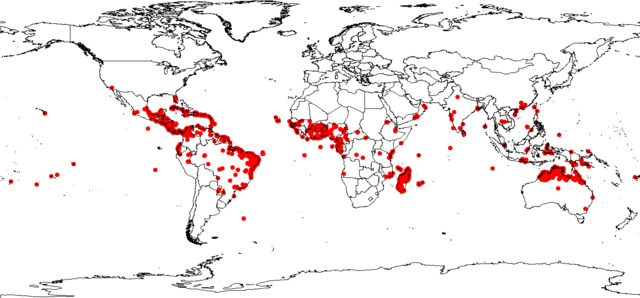
\includegraphics[width=4in,height=\textheight]{./gbif.png}

Diversity data from ebird or any citizen science project.

\hypertarget{humans}{%
\chapter{Human data}\label{humans}}


\includegraphics[width=4in,height=\textheight]{./humans.png}

Data associated with humans. Fitbit steps and sleep.

\hypertarget{rubrics}{%
\chapter{Rubrics}\label{rubrics}}

\hypertarget{experimental-designcraft-assessment-framework}{%
\subsubsection*{Experimental designcraft assessment framework}\label{experimental-designcraft-assessment-framework}}
\addcontentsline{toc}{subsubsection}{Experimental designcraft assessment framework}

There are at least two primary modes of assessment \citep{RN6795}. Formative assessment can happen during the learning process \citep{RN6796}. This active process of engagement with content and doing experiments is critical to becoming an effective life-long learner and successful scientist. In practicing experimental design and doing experiments professionally, this can take the of form of notes, sketches, photographs of the process or experiment at different steps, flowcharts, field and lab notebooks, code, and discussion with collaborators. This process of learning can include feedback from the team (in this course the teaching assistant, the instructor, or peers examining the same challenge). It can be enabled by testing how well one has advanced in achieving specific outcomes. For instance, share your meta-data with a peer and explore whether the individual can understand the meaning of the data and the process of experimentation that supported the collection or reuse of data. Summative assessment can happen at the end of key benchmarks in a learning cycle or at the completion of logical stopping points within the learning process that generated concrete products for review and grading \citep{RN6798}. In this designcraft process of actively exploring experimental design, this can include production of data with meta-data, a lab report describing the deeper dive for one of the field experiments, and a lab report describing the design process of data reuse from one the examples provided. The process of formative asessment (steps along the way) and summative assessment (final products) should support one another to consolidate learning \citep{RN6797}.

A rubric is a scoring tool that enables fair, transparent and replicable grading in summative evaluation \citep{RN6799}. Checklists are useful for formative self or peer assessment in the steps along the way to final products. In designcraft for experiments, this applies to the published data with meta-data and lab reports. In the formal offering of these labs for the course `SC/BIOL 3250 4.00 Experimental design for environmental and evolutionary biology' at York University, the lab component is worth 50\% of the final grade.

\hypertarget{lab-component-weightings}{%
\subsubsection*{Lab component weightings}\label{lab-component-weightings}}
\addcontentsline{toc}{subsubsection}{Lab component weightings}

Dataset with meta-data for pilot experiment 5\%\\
Dataset with meta-data for field experiment 5\%\\
Field lab report 30\%\\
Data-design lab report 10\%

\hypertarget{specific-rubrics}{%
\subsubsection*{Specific rubrics}\label{specific-rubrics}}
\addcontentsline{toc}{subsubsection}{Specific rubrics}

\hypertarget{formative-checklist-for-pilot-dataset}{%
\subsubsection*{Formative checklist for pilot dataset}\label{formative-checklist-for-pilot-dataset}}
\addcontentsline{toc}{subsubsection}{Formative checklist for pilot dataset}

This is not the marking key. This is a simple checklist to consider in doing the work or monitoring your progress in the process of doing the pilot experiment.

\begin{tabular}{rll}
\toprule
check & description & criteria\\
\midrule
1 & design & survey patterns locally, plan design\\
2 & identification & look up common species, explore field guides\\
3 & dataset & download, format, enter data\\
4 & principles & sketch design, take field notes\\
5 & principles & try different designs and sampling approaches\\
\addlinespace
6 & meta-data & note units and specifics of your data\\
7 & meta-data & take notes, plan how to write methods\\
8 & open science & explore figshare, check examples, set up account\\
9 & open science & publish data and meta-data\\
10 & innovation & consider how to improve and what different designs can test\\
\bottomrule
\end{tabular}

\hypertarget{formative-checklist-for-field-dataset}{%
\subsubsection*{Formative checklist for field dataset}\label{formative-checklist-for-field-dataset}}
\addcontentsline{toc}{subsubsection}{Formative checklist for field dataset}

This is not the marking key. This is a simple checklist to consider in doing the work or monitoring your progress in the process of doing the field experiment.

\begin{tabular}{rll}
\toprule
item & description & criteria\\
\midrule
1 & design & plan design\\
2 & dataset & plan a tidy dataset, ensure variables can test predictions\\
3 & meta-data & take detailed notes, record key techniques\\
4 & meta-data & get a peer to review data and meta-data\\
5 & open science & publish data and meta-data, ensure clear title, location, and details sufficient\\
\bottomrule
\end{tabular}

\hypertarget{summative-marking-key-for-published-datasets}{%
\subsubsection*{Summative marking key for published datasets}\label{summative-marking-key-for-published-datasets}}
\addcontentsline{toc}{subsubsection}{Summative marking key for published datasets}

This is the marking key you are looking for. This same key is used for both the pilot and field datasets to ensure that you can improve and learn from the process.

\begin{tabular}{rllr}
\toprule
item & description & criteria & score\\
\midrule
1 & data & tidy, clear labels, no errors & 1\\
2 & data & observations meaningful, accuracy, sufficient & 1\\
3 & meta-data & every variable or column clearly described & 1\\
4 & meta-data & description ensures the process of observation be repeated by another & 1\\
5 & open science & published data with meta-data, ensure clear title, location, and details sufficient & 1\\
\bottomrule
\end{tabular}

\hypertarget{formative-checklist-for-field-report}{%
\subsubsection*{Formative checklist for field report}\label{formative-checklist-for-field-report}}
\addcontentsline{toc}{subsubsection}{Formative checklist for field report}

This is a checklist to consider in writing up the field lab report.

\begin{tabular}{rll}
\toprule
check & description & criteria\\
\midrule
1 & design & explore system and reuse pilot experiment\\
2 & identification & examine a key driver within the system\\
3 & research & check the publish literature on the topic\\
4 & plan & write hypothesis and predictions\\
5 & data & collect your field data\\
\addlinespace
6 & test & test your data with plots and statistics\\
7 & confirm & validate your findings with logic and published science\\
8 & plot & make a single clear plot of data that summarizing key finding\\
9 & write & write up paper\\
10 & conclusions & explain the relevance of finding and make a clear conclusion\\
\bottomrule
\end{tabular}

\hypertarget{summative-assessment-marking-key-for-field-lab-report}{%
\subsubsection*{Summative assessment marking key for field lab report}\label{summative-assessment-marking-key-for-field-lab-report}}
\addcontentsline{toc}{subsubsection}{Summative assessment marking key for field lab report}

This is the marking key for the field lab report. Single spaced, 12 point font, at least 1 inch margins (the default). PDF format only. Lab reports must also be submitted to \href{https://www.turnitin.com}{turnitin.com} .

\href{https://www.facetsjournal.com/authors/instructions/}{Facets journal} is Canada's first and only multidisciplinary open access science journal. Follow the instructions proposed for a research article for this journal - \textbf{5000 words preferred}.

\begin{tabular}{lllr}
\toprule
page & concept & description & value\\
\midrule
1 & Title \& abstract & Title of experiment, your name, contact details, abstract that describes experiment & 5\\
2-3 & Introduction & Sets the context, explains why study needs to be done, state hypothesis and predictions & 5\\
4 & Methods & Decribed well enough for someone else to replicate design & 5\\
5 & Results & Clear text should be able to stand alone including description of statistics & 5\\
6-7 & Discussion & Restate findings in brief and then propose significance of the work & 5\\
\addlinespace
8 & Literature cited & At least 5 recent papers on topic and 2 on design decisions & 0\\
9 & Figure legend & Figure legend describing what the figure shows. & 2\\
10 & Figure & Figure on a single page & 3\\
\bottomrule
\end{tabular}

\hypertarget{formative-checklist-for-data-design-report}{%
\subsubsection*{Formative checklist for data-design report}\label{formative-checklist-for-data-design-report}}
\addcontentsline{toc}{subsubsection}{Formative checklist for data-design report}

This is a checklist to consider in writing up the field lab report.

\begin{tabular}{rll}
\toprule
check & description & criteria\\
\midrule
1 & design & explore data and look for patterns\\
2 & identification & imagine variables that can become key factors\\
3 & research & check the publish literature on the topic\\
4 & plan & write hypothesis and predictions\\
5 & test & test the data with plots and statistics\\
\addlinespace
6 & check & do you have what you need or do you need other data\\
7 & learn & check short research note papers to see style and writing\\
8 & plot & make a single clear plot of data that summarizing key finding\\
9 & write & write up paper\\
10 & innovation & list ideas for future experiments and implications\\
\bottomrule
\end{tabular}

\hypertarget{summative-assessment-marking-key-for-data-design-lab-report}{%
\subsubsection*{Summative assessment marking key for data-design lab report}\label{summative-assessment-marking-key-for-data-design-lab-report}}
\addcontentsline{toc}{subsubsection}{Summative assessment marking key for data-design lab report}

This is the marking key for the data-design short report. Single spaced, 12 point font, at least 1 inch margins (the default). PDF format only. Lab reports must also be submitted to \href{https://www.turnitin.com}{turnitin.com}.

\href{https://www.facetsjournal.com/authors/instructions/}{Facets journal} is Canada's first and only multidisciplinary open access science journal. Follow the instructions proposed for a note for this journal - \textbf{1400 words preferred}.

\begin{tabular}{rllr}
\toprule
page & concept & description & value\\
\midrule
1 & Title & Title of experiment, your name, contact details & 0\\
2 & Introduction & Single paragraph stating background, hypothesis, and your prediction(s) & 3\\
3 & Results & Single brief paragraph stating findings and single figure with legend & 5\\
4 & Conclusions & Single paragraph stating conclusion and implications & 2\\
5 & Lit cited & A total of 3 references & 0\\
\bottomrule
\end{tabular}

\hypertarget{notes}{%
\chapter{Final notes}\label{notes}}

Observations and conclusions.

  \bibliography{book.bib,packages.bib}

\end{document}
